% Generado por floyd.c
\documentclass[a4paper,11pt]{article}
\usepackage[utf8]{inputenc}
\usepackage{tikz}
\usepackage{array}
\usepackage[table]{xcolor}
\usepackage{longtable}
\usepackage{geometry}
\geometry{margin=1.5cm}
\begin{document}
\begin{center}
{\LARGE \textbf{Proyecto 1: Rutas Óptimas (Algoritmo de Floyd)}}\\[2cm]
{\large Investigación de Operaciones\\[2cm]
{\large Integrantes: }\\[1cm]
{\large Jose Pablo Fernandez Jimenez - 2023117752}\\[1cm]
{\large Diego Durán Rodríguez - 2022437509}\\[2cm]
{\large Segundo semestre 2025\\[1cm]
\end{center}
\newpage
\section*{Algoritmo de Floyd}


     Robert W. Floyd nació el 8 de junio de 1936 en New York, Estados Unidos y falleció el 25 de septiembre de 2001. Fue un importante científico de la computación y recibió un Turing Award en 1978 por sus contribuciones a la teoría de lenguajes de programación, algoritmos y estructuras de datos. Estudió Artes Liberales y Física en la Universidad de Chicago y realizó publicaciones muy influyentes en el campo de la informática. Uno de sus trabajos más importantes fue el desarrollo del algoritmo de Floyd-Warshall en 1962~\cite{hosch2024}.

El algoritmo de Floyd es un algoritmo de grafos con el cual se puede encontrar la ruta más corta entre todos los pares de nodos en un grafo ponderado. Este algoritmo tiene complejidad temporal $O(n^3)$ y espacial $O(n^2)$, donde $n$ es el número de nodos en el grafo. Para llevar a cabo el cálculo de la ruta más corta, el algoritmo utiliza dos matrices: una matriz de distancias (D) y una matriz de predecesores (P), que muestra el camino más corto~\cite{mukhopadhyay2023}.

\bigskip
\section*{Problema}
\begin{center}
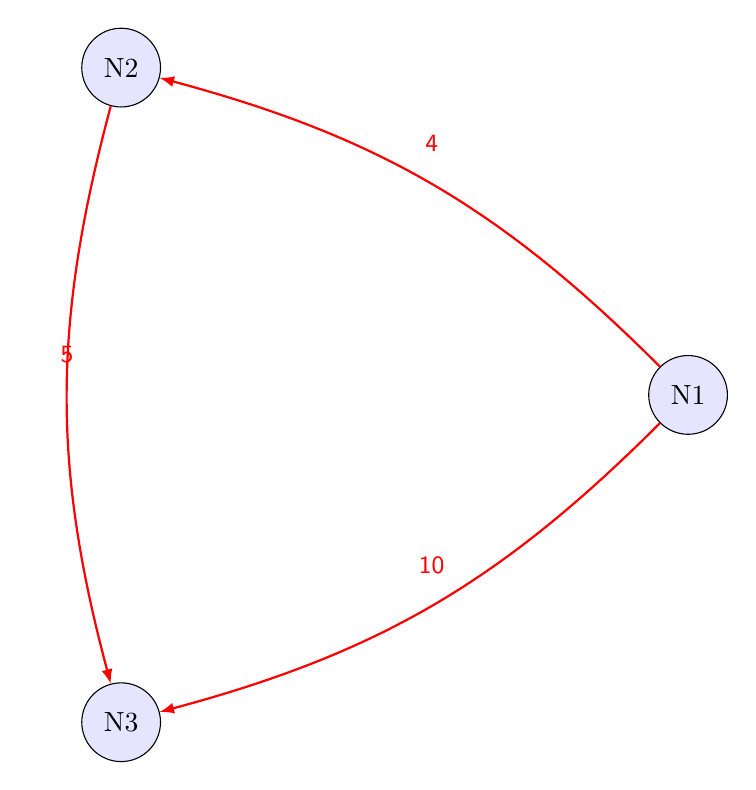
\begin{tikzpicture}[scale=1.2,
  every node/.style={circle, draw, fill=blue!10, minimum size=10mm},
  every edge/.style={draw, thick}]
\node (N0) at (4.000, 0.000) {N1};
\node (N1) at (-2.000, 3.464) {N2};
\node (N2) at (-2.000, -3.464) {N3};
\draw[->, thick, >=latex, red] (N0) to[bend right=15] node[midway, above, draw=none, fill=none, rectangle, font=\small\sffamily] {4} (N1);
\draw[->, thick, >=latex, red] (N0) to[bend left=15] node[midway, above, draw=none, fill=none, rectangle, font=\small\sffamily] {10} (N2);
\draw[->, thick, >=latex, red] (N1) to[bend right=15] node[midway, above, draw=none, fill=none, rectangle, font=\small\sffamily] {5} (N2);
\end{tikzpicture}
\end{center}
\newpage
\section*{Tablas iniciales}
\subsection*{D(0)}
\begin{center}
\begin{tabular}{c|ccc}
 & N1 & N2 & N3 \\ \hline
N1 & 0 & 4 & 10 \\
N2 & $\infty$ & 0 & 5 \\
N3 & $\infty$ & $\infty$ & 0 \\
\end{tabular}
\end{center}
\subsection*{P(0)}
\begin{center}
\begin{tabular}{c|ccc}
 & N1 & N2 & N3 \\ \hline
N1 & 0 & 0 & 0 \\
N2 & 0 & 0 & 0 \\
N3 & 0 & 0 & 0 \\
\end{tabular}
\end{center}
\newpage
\section*{Tablas intermedias}
\section*{Cálculo de D(1)}
\subsection*{D(1)}
\begin{center}
\begin{tabular}{c|ccc}
 & N1 & N2 & N3 \\ \hline
N1 & 0 & 4 & 10 \\
N2 & $\infty$ & 0 & 5 \\
N3 & $\infty$ & $\infty$ & 0 \\
\end{tabular}
\end{center}
\subsection*{P(1)}
\begin{center}
\begin{tabular}{c|ccc}
 & N1 & N2 & N3 \\ \hline
N1 & 0 & 0 & 0 \\
N2 & 0 & 0 & 0 \\
N3 & 0 & 0 & 0 \\
\end{tabular}
\end{center}
\newpage
\section*{Cálculo de D(2)}
\subsection*{D(2)}
\begin{center}
\begin{tabular}{c|ccc}
 & N1 & N2 & N3 \\ \hline
N1 & 0 & 4 & \textcolor{orange}{9} \\
N2 & $\infty$ & 0 & 5 \\
N3 & $\infty$ & $\infty$ & 0 \\
\end{tabular}
\end{center}
\subsection*{P(2)}
\begin{center}
\begin{tabular}{c|ccc}
 & N1 & N2 & N3 \\ \hline
N1 & 0 & 0 & N2 \\
N2 & 0 & 0 & 0 \\
N3 & 0 & 0 & 0 \\
\end{tabular}
\end{center}
\newpage
\section*{Cálculo de D(3)}
\subsection*{D(3)}
\begin{center}
\begin{tabular}{c|ccc}
 & N1 & N2 & N3 \\ \hline
N1 & 0 & 4 & 9 \\
N2 & $\infty$ & 0 & 5 \\
N3 & $\infty$ & $\infty$ & 0 \\
\end{tabular}
\end{center}
\subsection*{P(3)}
\begin{center}
\begin{tabular}{c|ccc}
 & N1 & N2 & N3 \\ \hline
N1 & 0 & 0 & N2 \\
N2 & 0 & 0 & 0 \\
N3 & 0 & 0 & 0 \\
\end{tabular}
\end{center}
\newpage
\section*{Distancias y rutas \'optimas}
\begin{longtable}{c c c p{7cm}}
\hline
Origen & Destino & Distancia & Ruta \\\hline
\endhead
N1 & N2 & 4 & N1 -- N2 \\
N1 & N3 & 9 & N1 -- N2 -- N3 \\
N2 & N1 & $\infty$ & (no existe ruta) \\
N2 & N3 & 5 & N2 -- N3 \\
N3 & N1 & $\infty$ & (no existe ruta) \\
N3 & N2 & $\infty$ & (no existe ruta) \\
\hline
\end{longtable}
\renewcommand{\refname}{Referencias}
\begin{thebibliography}{9}
\bibitem{hosch2024} Hosch. W. (2024). Robert W. Floyd. Encyclopedia Britannica. \\ \url{https://www.britannica.com/biography/Robert-W-Floyd}
\bibitem{mukhopadhyay2023} Mukhopadhyay, P. (2023). Floyd-Warshall Algorithm. Medium. \\ \url{https://medium.com/@mukhopadhyaypushan42/floyd-warshall-algorithm-7f09533b1878}
\end{thebibliography}
\end{document}
